\claude{
\section{Monitoring and selection in learned systems}\label{sec:applied}

\subsection{Detecting restricted parameter updates}\label{sec:cnn}
Can weight norm reveal that a classifier's updates now occupy fewer directions? We freeze layers, prune weights, or lower the learning rate in a CIFAR-10 classifier \citep{krizhevsky2009learning}. Comparisons use unchanged training, larger batches, and unchanged logs rescaled or smoothed after recording.

We look for a sustained drop in MG of the weight-norm log. On development runs we set the threshold above the largest drop in the controls and choose the block lengths that detect the most interventions. The resulting rule raises an alarm when median MG in the latest two windows is more than $8.83\%$ below the median of the preceding three (Equation~\ref{eq:detector}).

We count a detection if the first alarm comes within 5,000 updates after the intervention. This happened in 27 of 28 evaluation runs across seven strong interventions. The miss was one tenfold learning-rate reduction, and none of the comparison records triggered an alarm. Absolute successive changes detected as many interventions sooner, and normalized increments detected them all (Tables~\ref{tab:decisions} and~\ref{tab:detectors}).

In ResNet-18 \citep{he2016deep}, freezing the feature extractor leaves only the final classification layer trainable. MG falls along with the covariance PR of the weight updates (Figure~\ref{fig:resnet-freeze-trace}). The same rule detects every freeze with random or ImageNet initialization, but misses pruning and learning-rate reductions (\appref{app:applied}).

\begin{figure*}[!htb]
\centering
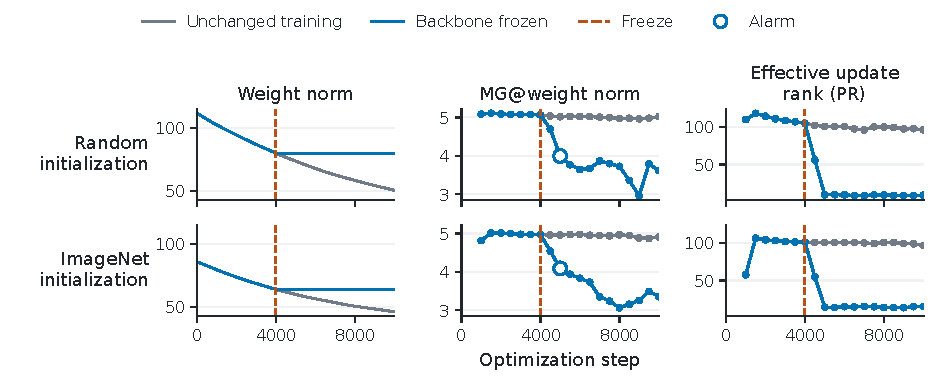
\includegraphics[width=.96\textwidth]{figures/resnet_freeze_trace.pdf}
\caption{Freezing the feature extractor in ResNet-18. Each column compares runs from the same starting weights, aligned at the intervention. The lower panels show how widely the updates vary across directions (update covariance PR). Points are placed at window ends.}
\label{fig:resnet-freeze-trace}
\end{figure*}

\FloatBarrier
\subsection[Tracking sentence information in a text VAE]{\cx{Tracking sentence information in a text VAE}}\label{sec:vae}
\cx{In a text variational autoencoder (VAE), the encoder maps each sentence $x$ to an approximate posterior $q(z\mid x)$ over a sentence-level latent variable $Z$. The decoder predicts each word from a sampled vector $z$ and the preceding words} \citep{bowman2016generating}. \cx{If the preceding words suffice for prediction, reconstruction loss can stay low even as the decoder becomes less sensitive to $z$.} Can the loss history reveal that change?

Starting from the same Penn Treebank model within each repeat \citep{marcus1993building}, we vary the penalty on the Kullback--Leibler (KL) divergence between \cx{$q(z\mid x)$ and the standard normal prior. A stronger penalty encourages the posteriors for different sentences to approach the same prior.} We also test \emph{free~bits}, which lets the batch-average KL of each \cx{latent dimension} rise to a threshold before the penalty increases \citep{kingma2016improved}.

\cx{We estimate how much information $Z$ carries about the input sentence $X$ using mutual information $I(X;Z)$. For each draw $z$ from $q(z\mid x)$, we compare its density under that sentence's posterior with its density under the mixture of posteriors across evaluation sentences. We average the log density ratio over draws and sentences (Equation~\eqref{eq:vae-mi}). To measure decoder sensitivity to $z$, we keep the preceding words fixed and measure how much the predicted word distribution changes when we draw $z$ from another sentence's posterior.}

\begin{figure*}[!htb]
\centering
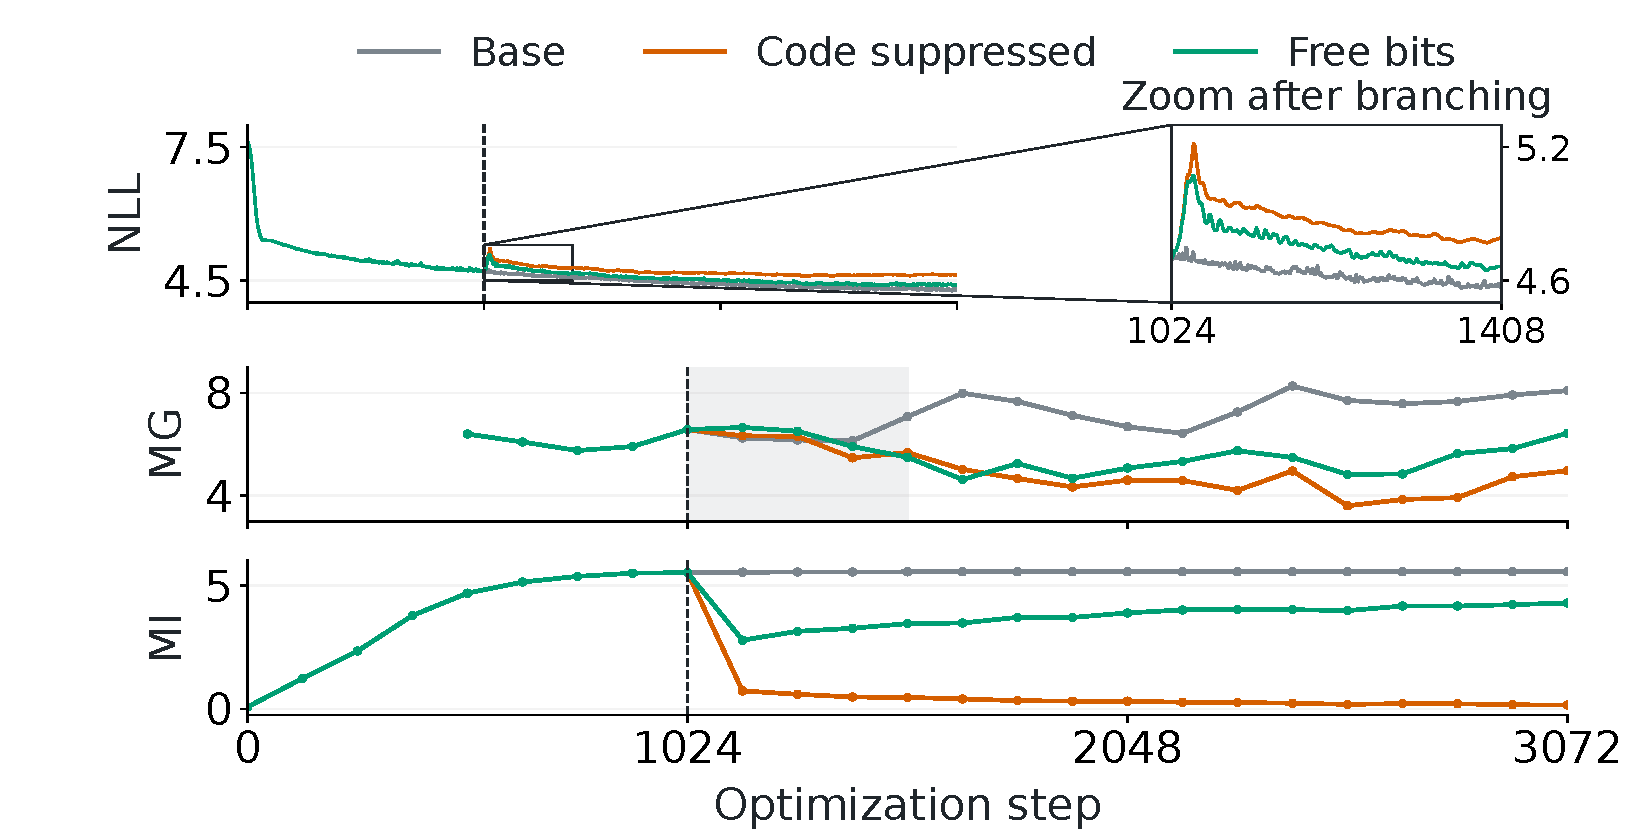
\includegraphics[width=.96\textwidth]{../poster/figures/vae_real_log.pdf}
\caption{\cx{Reconstruction loss, MG and sentence information during text VAE training.} NLL is the mean negative log-likelihood per token on fixed sentences. \cx{The bottom panel shows mutual information $I(X;Z)$ in nats.} The vertical line marks when the three penalty conditions begin. Shading extends to the end of the first MG window recorded entirely under the new setting.}
\label{fig:vae-loss-log}
\end{figure*}

Here we compare conditions over the final training interval. In each repeat we divide median MG of fixed-sentence loss under the stronger penalty by its median under the weaker penalty. The median ratio across nine repeats is 0.52. \cx{Mean loss changes little, while mutual information and decoder sensitivity both fall.} Free bits partly preserves sentence information and MG (Figure~\ref{fig:vae-loss-log} and Table~\ref{tab:vae-mg-ratios}). Standard deviation and spectral entropy of the loss also fall in every repeat (\appref{app:vae-information}).

\subsection{Warning of transformer loss spikes}\label{sec:spike-warning}
As a transformer learns modular addition, its loss can spike abruptly. We compare warning rules on development runs, maximizing the number of spikes warned of subject to at most two false alarms per 10,000 scored updates. The selected rule checks every 50 updates and warns when MG of the latest 500 log losses is at or below 6.3144 (rounded). A spike counts as detected if at least one warning occurs in the 500 updates before its onset. This rule warned of 22 of 23 evaluation spikes, including the one in Figure~\ref{fig:slingshot-warning} with 195 updates to spare. Roughness, the standard deviation of successive log-loss differences divided by that of the log losses, warned of all 23 at the same evaluation false-alarm rate (Table~\ref{tab:spikes_campaign}).

\begin{figure*}[!htb]
\centering
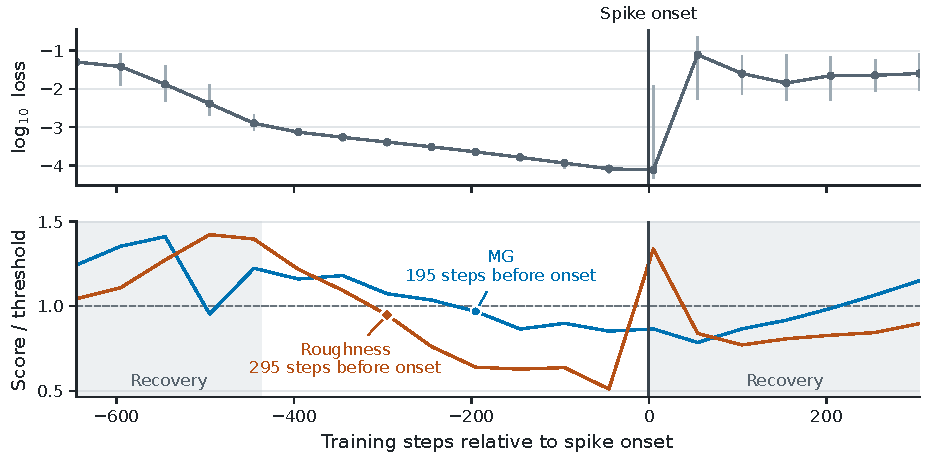
\includegraphics[width=.92\textwidth]{figures/slingshot_warning.pdf}
\caption{A loss spike in an evaluation run. The top band shows the minimum and maximum log loss around the mean in each block. Blue shading marks the interval for successful warnings. Dotted lines show the thresholds chosen on development runs. Dots mark the first warnings.}
\label{fig:slingshot-warning}
\end{figure*}

\Needspace{7\baselineskip}
\subsection[Model selection from scalar logs]{Model selection from scalar logs}\label{sec:ssl}
We train image encoders on different views of each MNIST digit without using its label. To score an encoder, we freeze it and train a linear digit classifier on its features. On two development repeats we choose the scalar log and ranking direction with the highest mean Spearman correlation with classifier accuracy. The resulting rule picks the encoder with the highest MG over its final 1,000 gradient norms. Across five new repeats its choice averages 0.41 percentage points below the best of 29 configurations. A statistic using features from many images ranks the full set slightly better (Figure~\ref{fig:ssl-probe-scatter} and Table~\ref{tab:ssl_campaign}).

\paragraph{\cx{Forecast model choice.}}\label{sec:forecast_utility}
\cx{To forecast one neuron's activity, we need to choose a model from the observations so far. Testing every candidate on earlier parts of the record takes time. We ask whether MG of the observed activity can guide the choice. Figure~\ref{fig:single-neuron-forecasts} shows cases where MG and held-out search choose different models. The two selection methods yield similar mean forecast errors, with substantial uncertainty about the gap (Table~\ref{tab:forecast_all}).}

\cx{Computing MG at a subset of delay vectors preserves every model choice in this evaluation and reduces selection time below held-out search on the same inputs (Table~\ref{tab:forecast_utility}).}

\begin{table}[htbp]
\centering\small
\caption{\cx{Forecast error and selection time. NMSE uses prefix variance and is mean $\pm$ SD across 20 repeats after averaging tasks within each repeat. Time is the median on matched inputs.}}
\label{tab:forecast_utility}
\begin{tabularx}{\linewidth}{@{}>{\raggedright\arraybackslash}Xrr@{}}
\toprule
Selection rule & NMSE & Time (ms) \\
\midrule
MG, all queries (KD-tree) & $0.0364\,\pm 0.0213$ & 199.1 \\
\cx{MG, 128 queries (direct distance calculation)} & $0.0364\,\pm 0.0213$ & 12.2 \\
Lowest validation error & $0.0407\,\pm 0.0324$ & 45.3 \\
\bottomrule
\end{tabularx}

\end{table}

\begin{figure*}[htbp]
\centering
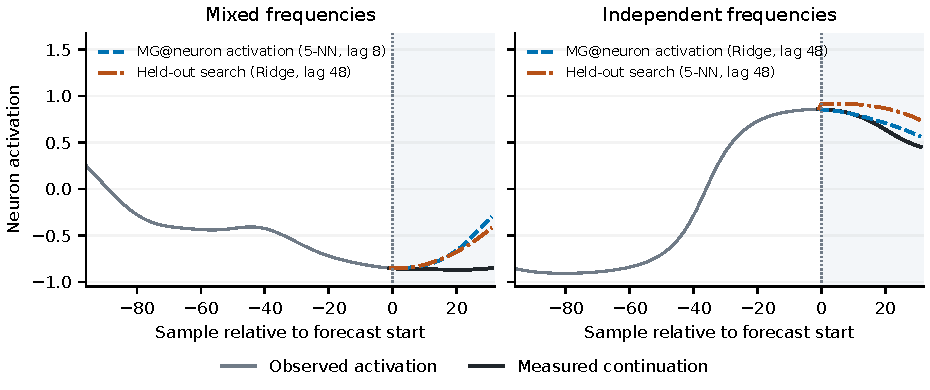
\includegraphics[width=.96\textwidth]{figures/single_neuron_forecasts.pdf}
\caption{\cx{Forecasts from the same held-out repeat. The plots show the end of the observed prefix. Held-out search is closer on the mixed-frequency target, and MG selects the closer forecast on the independent-frequency target.}}
\label{fig:single-neuron-forecasts}
\end{figure*}

}
